\section{Plateau de jeu}
\subsection{Tuiles}
En observant la forme des tuiles de Carcassonne,on peut remarquer que chaque tuile est caractériser par 13 positions Comme l’illustre la figure \ref{positions tuiles}, 3 sur chaque côté et une au centre:

\begin{figure}[h]
     \begin{minipage}{0.48\textwidth}
    \centering
    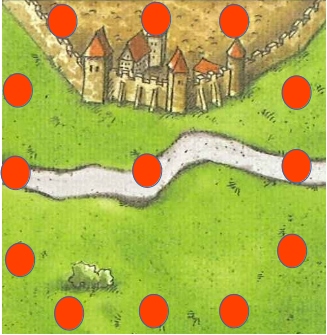
\includegraphics[width=0.6\textwidth,height=3.5cm]{images/tile1.png}
    \end{minipage}\hfill
    \begin{minipage}{0.48\textwidth}
    \centering
    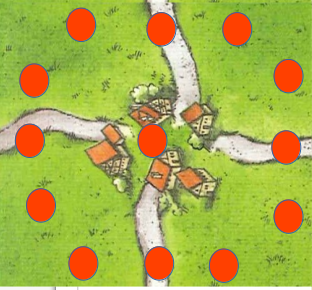
\includegraphics[width=0.6\textwidth,height=3.5cm]{images/tile2.png}
    \end{minipage}
    \caption{Les positions qui caractérisent les tuiles de Carcassonne}
    \label{positions tuiles}
\end{figure}
cela nous donne une idée pour définir une structure des tuiles. Comme le jeu contient un nombre fini d'objets (ville,route,champ,abbaye),on peut donc associer  à chaque objet une couleur. Par exemple,marron pour les villes,vert pour les champs,gris pour les routes...etc. Finalement toute tuile peut être représenté par la structure \textit{struct tile\_t} suivante:

\[
\text{struct tile\_t} \left\{
\begin{array}{l}
\text{t} \quad \rightarrow \quad \text{tableau d'entiers de taille 13}\\
\text{c} \quad \rightarrow \quad \text{tableau de couleurs de taille 13}\\
\end{array}
\right.
\]

\subsection{Pioche}
La pioche sera représentée par un type abstrait de données \textit{struct deck\_t}, dont l'implémentation dans le fichier deck.c contient trois champs:
\begin{itemize}
    \item deck qui un pointeur pointant sur les tuiles et qui sera alloué dynamiquement.
    \item size qui indique le nombre de tuiles stockées.
    \item capacity qui indique la taille de la mamoire allouée.
\end{itemize}
\[
\text{struct deck\_t} \left\{
\begin{array}{l}
\text{deck} \quad \rightarrow \quad \text{un poiteur pointant sur un tableau de tuiles }\\
\text{size} \quad \rightarrow \quad \text{entier}\\
\text{capacity} \quad \rightarrow \quad \text{entier}\\
\end{array}
\right.
\]
\subsection{Plateau}
\subsubsection{Plateau est un TAD }
Le plateau peut être implémenté de diverses façons, telles qu'une matrice ou une liste chaînée. Par conséquent, il est essentiel que la structure du Plateau soit un type abstrait de données, ce qui permet de rendre son implémentation plus flexible et indépendante du reste du code. \\
Pour représenter le plateau, une méthode simple consiste à utiliser une matrice de taille 2N, où N correspond au nombre total de tuiles. Cette approche offre plusieurs avantages, notamment un accès aux éléments du plateau en temps constant. Toutefois, cette méthode présente un inconvénient majeur : sa complexité en espace est de O($N^2$), ce qui est très coûteux en termes de mémoire.

Une deuxième méthode consiste à représenter le plateau par un tableau de taille N avec N le nombre de tuiles totales. Bien qu'il soit évident que cette méthode augmente la complexité en temps de certaines primitives, elle garantit une complexité linéaire en termes d'espace. Comme nous le verrons par la suite, la plupart des algorithmes associés à cette méthode sont linéaires, rendant cette approche plus envisageable.

Désormais, nous allons détailler la conception de la deuxième méthode.
\subsubsection{Tuiles dans le plateau}
\subsubsection*{Stockage des tuiles}
Stocker l'intégralité des tuiles dans le plateau augmenterait considérablement la complexité en espace. De plus, le nombre de tuiles différentes est fini. Par conséquent, nous pouvons stocker toutes les tuiles possibles dans un tableau \textbf{TILES\_TYPE}. Ainsi, nous pourrons stocker les tuiles dans le plateau en utilisant uniquement leurs indices dans \textbf{TILES\_TYPE}.
\subsubsection*{Rotation des tuiles}
Pendant la partie, la rotation des tuiles est autorisée. Il est donc nécessaire de savoir comment chaque tuile a été orientée. Pour ce faire, nous ajoutons un deuxième champ qui détermine l'orientation de la tuile sur le plateau.
\subsubsection*{Coordonnées et voisines d'une tuile}
Pour poser une tuile, il est nécessaire de connaître sa position aprés, ce qui rend indispensable l'ajout d'un champ déterminant cette position. Jusqu'à présent, le plateau présente un inconvénient majeur : pour passer d'une tuile à sa voisine, il faut parcourir à nouveau le tableau du plateau. Pour remédier à ce problème, nous pouvons ajouter des informations supplémentaires à chaque tuile concernant ses voisines en stockant leurs identifiants. Finalement les tuiles stockées dans le plateau vont avoir la stucture \textbf{struct status} suivante:
\[
\text{struct status} \left\{
\begin{array}{l}
\text{type\_id} \quad \rightarrow \quad \text{un entier indiquant le type de la tuile }\\
\text{rotation} \quad \rightarrow \quad \text{entier indiquant l'orientation de la tuile}\\
\text{x,y} \quad \rightarrow \quad \text{deux entiers indiquant les coordonnées }\\
\text{neighbors} \quad \rightarrow \quad \text{un tableau d'entier de taille 4  }\\
\end{array}
\right.
\]
Pour connaître précisément les identifiants de chaque voisine, il est nécessaire de les stocker de manière unique. Ainsi, chaque indice correspond à une direction spécifique. Nous choisissons respectivement les indices 0, 1, 2 et 3 pour représenter les directions nord, est, sud et ouest.\\
\textbf{Remarque}: Si une tuile ne possède pas de voisine dans une direction donnée, la valeur de cette voisine sera -1.
La figure \ref{two tiles} sera représenté par un tableau qui contient tile1 et tile2:
\begin{itemize}
    \item tile1=\{0,0,(0,0),{-1,-1,-1,1}\}
    \item tile2=\{1,0,(-1,0),{-1,0,-1,-1}\}
\end{itemize}
\begin{figure}[h]
    \centering
    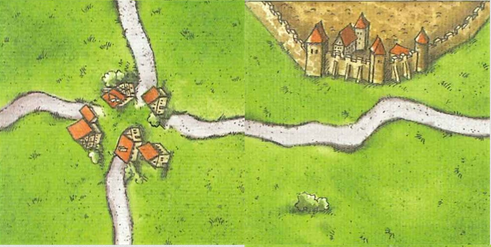
\includegraphics[width=0.8\textwidth]{images/tile125.png}
    \caption{deux tuiles du plateau}
    \label{two tiles}
\end{figure}
\subsubsection{Bords du plateau et graphe}
Même si le plateau est représenté par un tableau, il est initialement rempli de tuiles vides. Au fur et à mesure que la partie progresse, des tuiles sont ajoutées au plateau. C'est pourquoi il est nécessaire d'ajouter un champ \textbf{size} qui indique le nombre de tuiles jouées pendant la partie.\\

Pour déterminer les positions disponibles afin de poser une tuile sur le plateau, il faut d'abord identifier les positions sur le bord du plateau. Deux méthodes sont possibles :
\begin{itemize}
    \item À chaque fois qu'on veut jouer une tuile, on exécute une boucle qui recherche les positions sur le bord du plateau.
    \item On stocke les positions sur le bord du plateau dans une liste chaînée et à chaque fois, de nouvelles positions sont ajoutées à cette liste. 
\end{itemize}
En comparant les deux méthodes et compte tenu de la nature du jeu qui nécessite de jouer 72 tuiles, il est évident que la première méthode pourrait entraîner une complexité en temps considérable. Par conséquent, il est préférable d'utiliser la deuxième méthode, qui consiste à stocker les positions sur le bord du plateau dans une liste chaînée. 
On ajoute aussi  un autre champ graphe qui représente le graphe du plateau (il est détaillé dans la partie suivante),qui sert à calculer les composantes connexes afin de calculer le score.\\

Finalement la structure adoptée pour le plateau est la suivante :
\[
\text{struct board\_t} \left\{
\begin{array}{l}
\text{tiles} \quad \rightarrow \quad \text{un tableau de type struct tile\_t }\\
\text{size} \quad \rightarrow \quad \text{entier indiquant le nombre de tuile jouées}\\
\text{graph} \quad \rightarrow \quad \text{graphe de igraph }\\
\text{empty} \quad \rightarrow \quad \text{une liste chaînée de type struct tile\_t  }\\
\end{array}
\right.
\]
\subsection{Principales algorithmes du plateau}
Le plateau contient trois types de  fonctions:
\begin{itemize}
    \item \textbf{fonctions d'initialisation} : ces fonctions ont pour but d'allouer la mémoire pour le plateau, et de l'initialiser en ajoutant la coordonnée (0,0) au champ \textbf{empty} du plateau . Exemples: \textbf{Initialize\_board,Allocate\_board}.
    \item \textbf{fonctions de gestion de tuiles} :Ces fonctions permettent principalement d'ajouter les tuiles au plateau et de chercher une position valide pour chaque tuile. Exemples: \textbf{correct\_pasting, add\_tile, is\_corrected\_played}.
    \item \textbf{fonctions de gestion de empty} : ces fonctions garantissent l'ajout des nouvelles positions du bords du plateau ainsi que la suppression des positions occupées et le changement des identifiants des voisines de chaque tuile. Exemple:\textbf{ change\_neighbors}.
\end{itemize}
\subsubsection{Compléxité des alogrithmes}
soient N la taille de la structure \textit{board\_t} et \footnotesize {EMPTY\_SIZE} la taille de \textbf{empty}.
\begin{itemize}
    \item Les fonctions d'initialisation :Les fonctions \textbf{allocate\_board} et \textbf{initialize\_board} ont une complexité linéaire en temps et en espace, soit O(N), puisqu'elles se limitent à allouer la mémoire et à initialiser le champ \textbf{empty} du plateau.
    \item Les fonctions de gestion de tuiles : La fonction \textbf{correct\_pasting} accède à un élément de \textbf{empty}, qui est une liste chaînée, et effectue quatre appels à la fonction \textbf{flip\_tile}, qui fait pivoter les tuiles. Par conséquent, sa complexité est O(\footnotesize{MAX\_CONNECTIONS + EMPTY\_SIZE}), où \footnotesize{MAX\_CONNECTIONS} représente la taille des deux tableaux d'une tuile.
    \item Les fonctions de gestion de empty: Les fonctions \textbf{change\_neighbors} et \textbf{get\_possible\_moves} ont une complexité linéaire en \footnotesize{EMPTY\_SIZE} car elles accèdent aux éléments de \textbf{empty} et en suppriment certains.
\end{itemize}
